% Don't Do That: Keep your data in line with database constraints

% XXX XXX XXX This talk is boring. It's listing all the ways you can do stuff,
% without engaging examples of why you'd want to

\documentclass{beamer}
\usetheme{Madrid}
% \usepackage[font=small,labelfont=bf]{caption}

\begin{document}
\title{Don't Do That}
\subtitle{Ensuring data sanity with database constraints}
\author{Joshua Tolley, End Point Corporation}

\frame{\titlepage}
%\frame{\tableofcontents}

%        \item Examples of index constraints (UNIQUE) (incl. partial, multicolumn, functional)
%        \item Postgresql exclusion constraints
%        \item triggers (note that these don't validate existing data)
%        \item Why am I not talking about rules?
%        \item Refute Rails' "The app does it for me, so I don't have to worry about it in the database" agnosticism

\begin{frame}{ACID}
    \begin{figure}[t]
        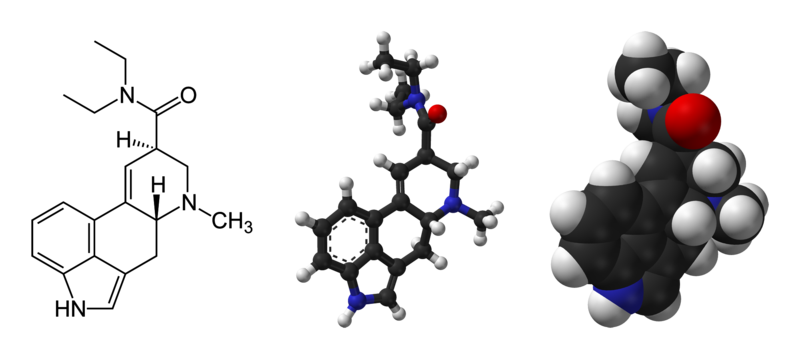
\includegraphics[width=0.8\textwidth]{lsd.png}
        \caption{Lysergic acid diethylamide, public domain image courtesy of Benjah-bmm27, Wikipedia}
    \end{figure}
\end{frame}

\begin{frame}{ACID}
    We've all heard about ACID:
    \begin{itemize}
        \item {\bf \color{red}Atomicity}: Operations are grouped into transactions; each transaction either succeeds or fails in its entirety
        \item {\bf \color{red}Consistency}: At the end of each transaction, the data meet all applicable constraints
        \item {\bf \color{red}Isolation}: Data from uncommitted transactions are invisible to all but the transaction that created them
        \item {\bf \color{red}Durability}: Kicking the power cord doesn't destroy your data
    \end{itemize}
    Most developers ignore atomicity and consistency, don't understand isolation, and take durability for granted.
\end{frame}

\begin{frame}{Just consistency, please}
    If you expect to hear about Atomicity, Isolation, or Durability, you're in the wrong room.
\end{frame}

\begin{frame}{Database constraints}
    You get consistency from database constraints. Constraints ensure your data remain sane, meaningful, and unambiguous. If you do them right.
\end{frame}

\begin{frame}
    \begin{block}{Why?}
        If you've ever dealt with "bad" data in the database, you'll understand why constraints are important
    \end{block}
\end{frame}

\begin{frame}{Database constraints}
    SQL databases maintain constraints in several ways:
    \begin{itemize}
        \item Check constraints
        \item Data type, including custom data types and domains
        \item UNIQUE, NOT NULL, DEFAULT (kinda)
        \item Primary and foreign keys
        \item Triggers
        \item Exclusion constraints
    \end{itemize}
\end{frame}

\begin{frame}[fragile]
    \frametitle{Check constraints}
    Check constraints simple verify a given expression
\small
    \begin{verbatim}
   CREATE TABLE foo (
       i INTEGER,
       j INTEGER,
       p FLOAT CHECK (p > 0),
       CHECK ( (i IS NULL) OR (j IS NULL))
   );

   hal=# \d foo
             Table "public.foo"
    Column |       Type       | Modifiers
   --------+------------------+-----------
    i      | integer          |
    j      | integer          |
    p      | double precision |
   Check constraints:
       "foo_check" CHECK (i IS NULL OR j IS NULL)
       "foo_p_check" CHECK (p > 0::double precision)
    \end{verbatim}
\end{frame}

\begin{frame}[fragile]
    \frametitle{Check constraints}
    \small
    \begin{verbatim}
   hal=# insert into foo (p) values (-10);
   ERROR:  new row for relation "foo" violates check constraint
       "foo_p_check"
   
   hal=# insert into foo (p) values (10);
   INSERT 0 1
   hal=# select * from foo;
    i | j | p
   ---+---+----
      |   | 10
   (1 row)
   
   hal=# update foo set i = 1;
   UPDATE 1
   hal=# update foo set j = 1;
   ERROR:  new row for relation "foo" violates check constraint
       "foo_check"
    \end{verbatim}
\end{frame}

\begin{frame}{Data types}
    Many data types include parameters of one sort or another. Most have
    inherent limitations that act as constraints.
    \begin{itemize}
        \item Integers are limited to a specific range, and have no fractional part
        \item VARCHAR() fields are often limited in length
        \item ENUM types can contain only values from a defined set
        \item Date and time types can contain only \bf{\color{red}VALID*} dates
        \item Geometric, network, and other more complex types are also constrained
    \end{itemize}
    \vspace{10mm}
    {\footnotesize \color{red} \emph{* MySQL, are you listening?}}
\end{frame}

\begin{frame}[fragile]
    \frametitle{Custom data types}
    Many databases allow users to define their own data types
    \begin{block}{Composite data type}
    \begin{verbatim}
   CREATE TYPE complex AS (
       r       double precision,
       i       double precision
   );
    \end{verbatim}
    \end{block}
    \begin{block}{User-defined data type}
    \begin{verbatim}
   CREATE TYPE box (
       INTERNALLENGTH = 16,
       INPUT = my_box_in_function,
       OUTPUT = my_box_out_function,
       ELEMENT = float4
   );
    \end{verbatim}
    \end{block}
\end{frame}

\begin{frame}[fragile]
    \frametitle{Domains}
    The SQL standard includes \emph{domains}, which combine a given data type
    with one or more check constraints (more on check constraints later).
    \begin{verbatim}
  CREATE DOMAIN us_postal_code AS TEXT
      CHECK(
          VALUE ~ '^\d{5}$'
          OR VALUE ~ '^\d{5}-\d{4}$'
  );
    \end{verbatim}
\end{frame}

\begin{frame}{Column constraints}
    Column definitions can include constraints:
    \begin{itemize}
        \item UNIQUE
        \item NULL / NOT NULL
        \item DEFAULT (not really a constraint, but common with NOT NULL fields)
        \item PRIMARY KEY
        \item REFERENCES ... (foreign keys)
        \item CHECK
    \end{itemize}
\end{frame}

\begin{frame}{UNIQUE, [NOT] NULL}
    \begin{itemize}
        \item Unique columns must contain unqiue values
        \item "Unique" depends on the data type's definition of equality
        \item NULL means "unknown", so NULL != NULL, so UNIQUE columns can contain multiple NULLs
        \begin{itemize}
            \item ...so you might consider including a NOT NULL
            \item ...and perhaps a DEFAULT
        \end{itemize}
    \end{itemize}
    \begin{block}{Note}
        In PostgreSQL, UNIQUE is implemented with an index
    \end{block}
\end{frame}

\begin{frame}{PRIMARY KEY}
    Primary keys are UNIQUE and NOT NULL. Tables may have only one primary key, but many UNIQUE + NOT NULL columns.
\end{frame}

\begin{frame}[fragile]
    \frametitle{FOREIGN KEY}
    \begin{verbatim}
CREATE TABLE foo (
    bar INTEGER REFERENCES baz (qux)
);
    \end{verbatim}
    \begin{block}{Note} In PostgreSQL, columns referenced in a foreign key must be declared UNIQUE
    \end{block}
\end{frame}

\begin{frame}
    \frametitle{FOREIGN KEY - Cascading}
    What happens when a value in a referenced table gets modified?
\end{frame}

\begin{frame}{FOREIGN KEY - Cascading}
    \texttt{ON UPDATE \emph{action}} and \texttt{ON DELETE \emph{action}}
    \begin{itemize}
        \item {\bf NO ACTION}: Throw an error saying that the action would break consistency
        \item {\bf RESTRICT}: Same as "NO ACTION", but not deferrable
        \item {\bf CASCADE}: Delete or update all rows referencing this row
        \item {\bf SET NULL}: Set referencing columns to NULL
        \item {\bf SET DEFAULT}: Set the referencing columns to their default values.
    \end{itemize}
\end{frame}

\begin{frame}{Multi-column constraints}
    These constraints can apply to multiple columns
    \begin{itemize}
        \item CREATE UNIQUE INDEX foo ON bar (baz, qux)
        \item CREATE TABLE CONSTRAINT foo\_fkey FOREIGN KEY (bar, baz) REFERENCES alpha (bar, baz)
    \end{itemize}
    \vspace{0.1\textheight}
    \begin{block}{Note}
        You can even set multi-column foreign keys so some of the columns can be NULL, but it's rarely used. Google "foreign key match clause" for more.
    \end{block}
\end{frame}

\begin{frame}{Triggers}
    Triggers run user-defined functions (UDFs) when various things happen. Details of UDF programming are beyond this talk, but here's an example
    \vspace{0.1\textheight}
    \begin{block}{Note}
        PostgreSQL has at least 18 different languages available for user-defined functions
    \end{block}
\end{frame}

\end{document}
